\chapter{Програмна реализация на система за прогнозиране}

На база на разгледаните алгоритми и системи за прогнозиране, изборът за изработка на софтуерна система за прогнозиране пада върху клиент-сървър базирана архитектура, в която мобилни устройства извършват изчисления на изчислими пакети. Изчисленията се организират под формата на дарена изчислителна мощност. 

\section{Архитектура на системата}

Най-обобщеното представяне на разработената система съдържа трите най-важни компонента – сървър, комуникационна среда и мобилни устройства (Фиг. \ref{fig0054}). Комуникационната среда е глобалната мрежа Интернет. Информацията, която трябва да бъде изчислена, основно се намира на специално предназначен за нуждите на системата сървър. Изчислителните възли в системата са умни мобилни устройства. 

Основна цел при разработването е крайното решение да бъде максимално икономически изгодно. Това означава, че разходите за поддържане на цялата инфраструктура трябва да бъдат минимизирани. Тази цел може да бъде постигната, ако разходите за поддържането на сървър бъдат снижени възможно най-много. Системата трябва да работи с маломощен сървър, който само да синхронизира пресмятанията и да съхранява получените междинни резултати. Тъй като потребителите в системата даряват техните изчислителни ресурси, практически разходите от страна на клиента са сведени до нула. Всеки потребител сам закупува мобилното си устройство, сам заплаща сметката за изразходвания Интернет трафик и сам заплаща електричеството, необходимо за опериране на устройството. Поради стремежа за минимално натоварен сървър, вместо закупуването на отделна сървър машина и разполагането й в информационен център, спокойно може да се наеме уеб услуга от тип споделен хостинг (Фиг. \ref{fig0055}). 

\begin{figure}[H]
  \centering
  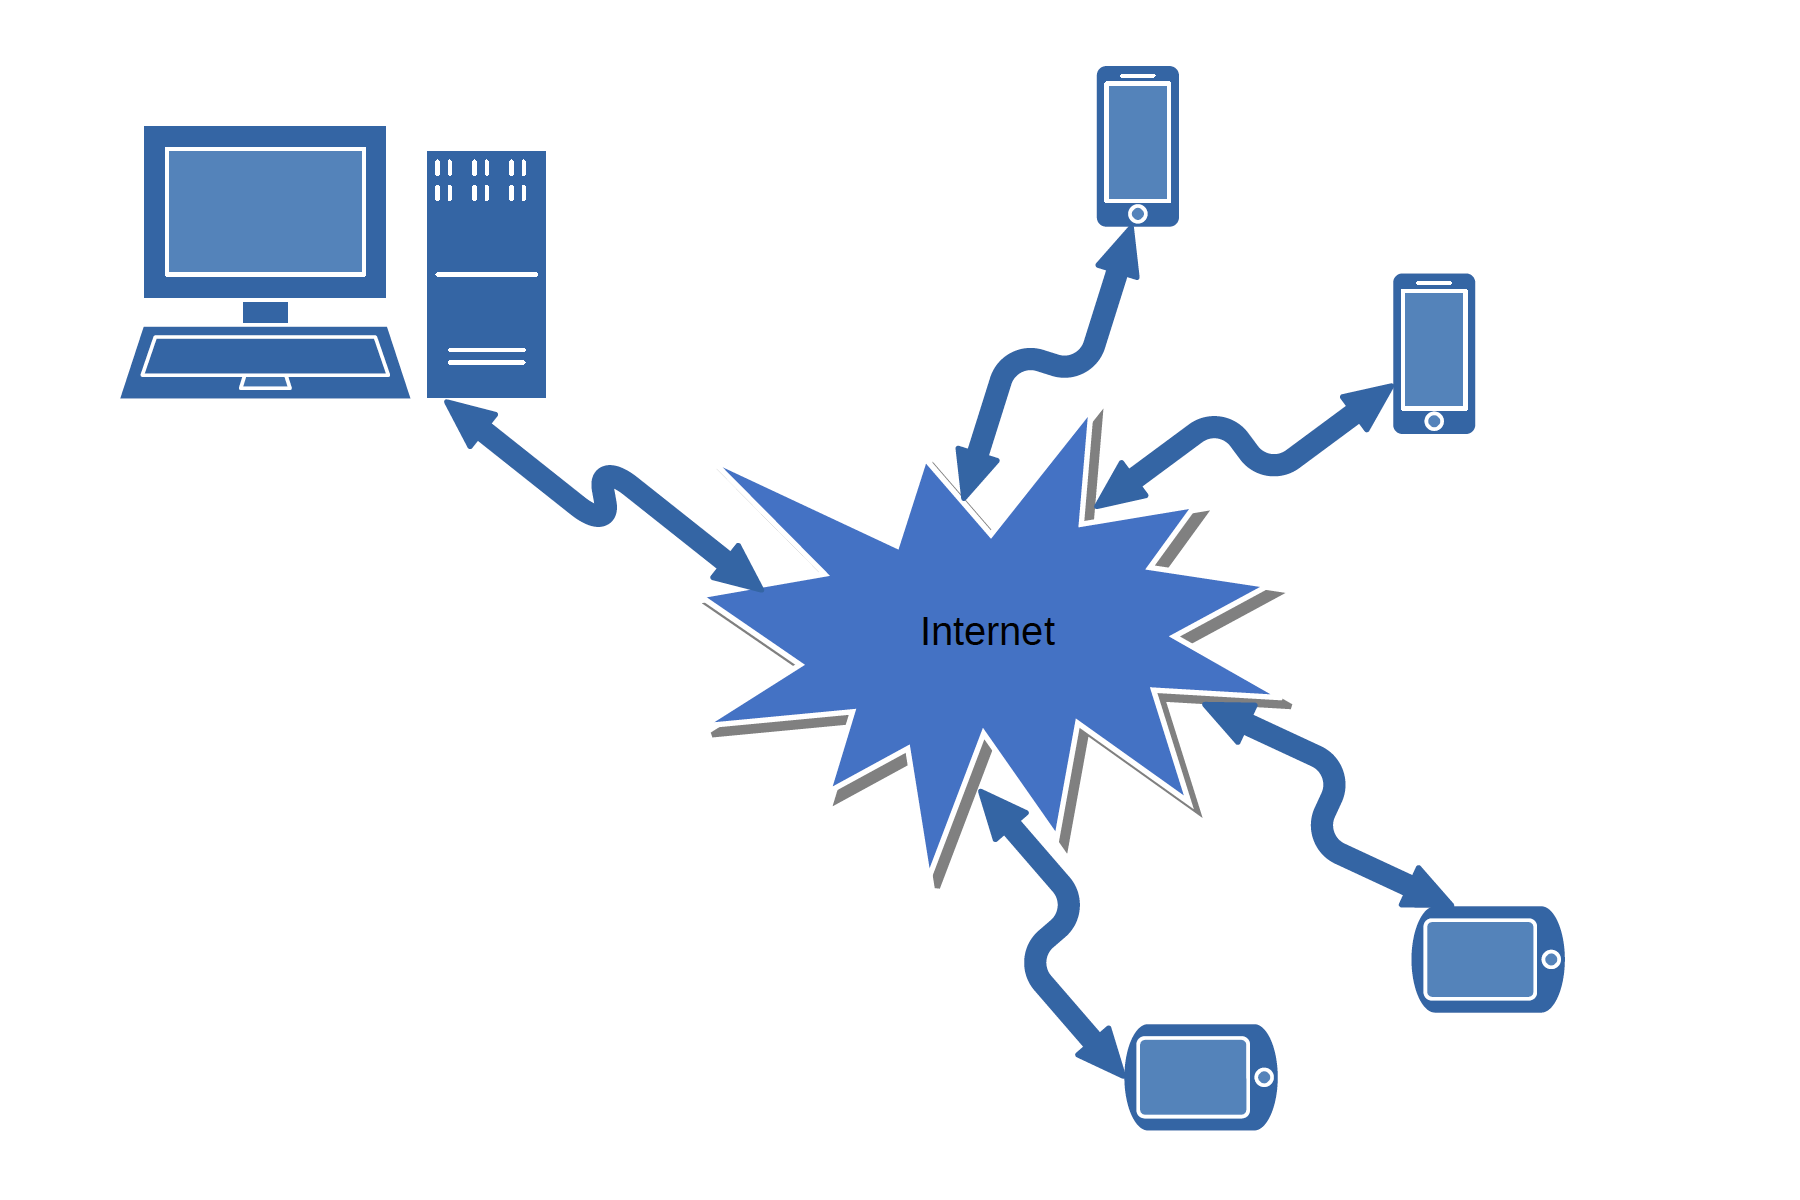
\includegraphics[width=0.8\linewidth]{fig0054.png}
  \caption{Обща организация на системата}
\label{fig0054}
\end{figure}

При споделения хостинг, върху една физическа машина доставчикът стартира множество виртуални машини и в самите виртуални машини се активират отделни инстанции на уеб сървърни приложения. Най-често използваните от доставчиците на споделен уеб хостинг операционни системи са базирани на Linux. Операционната система Linux много добре се съчетава с уеб сървъра Apache. Към уеб сървъра доставчиците най-често предлагат и MySQL релационна база данни. Apache уеб сървъра най-често има настроена поддръжка на PHP интерпретатора. Споделен хостинг в конфигурация Linux-Apache-MySQL-PHP (XAMPP) е едно от икономически най-ефективните решения. Като алтернативи може да се ползват Windows базирани сървъри, който поддържат MS SQL Serve база данни и ASP.NET уеб страници. Възможни са също комбинации с JSP, PostgreSQL или Oracle, но никоя от изброените комбинации не може да постигне икономическата ефективност на XAMPP. Споделеният хостинг при конфигурация XAMPP може да се наеме за абонамент от няколко долара на месец. 

\begin{figure}[H]
  \centering
  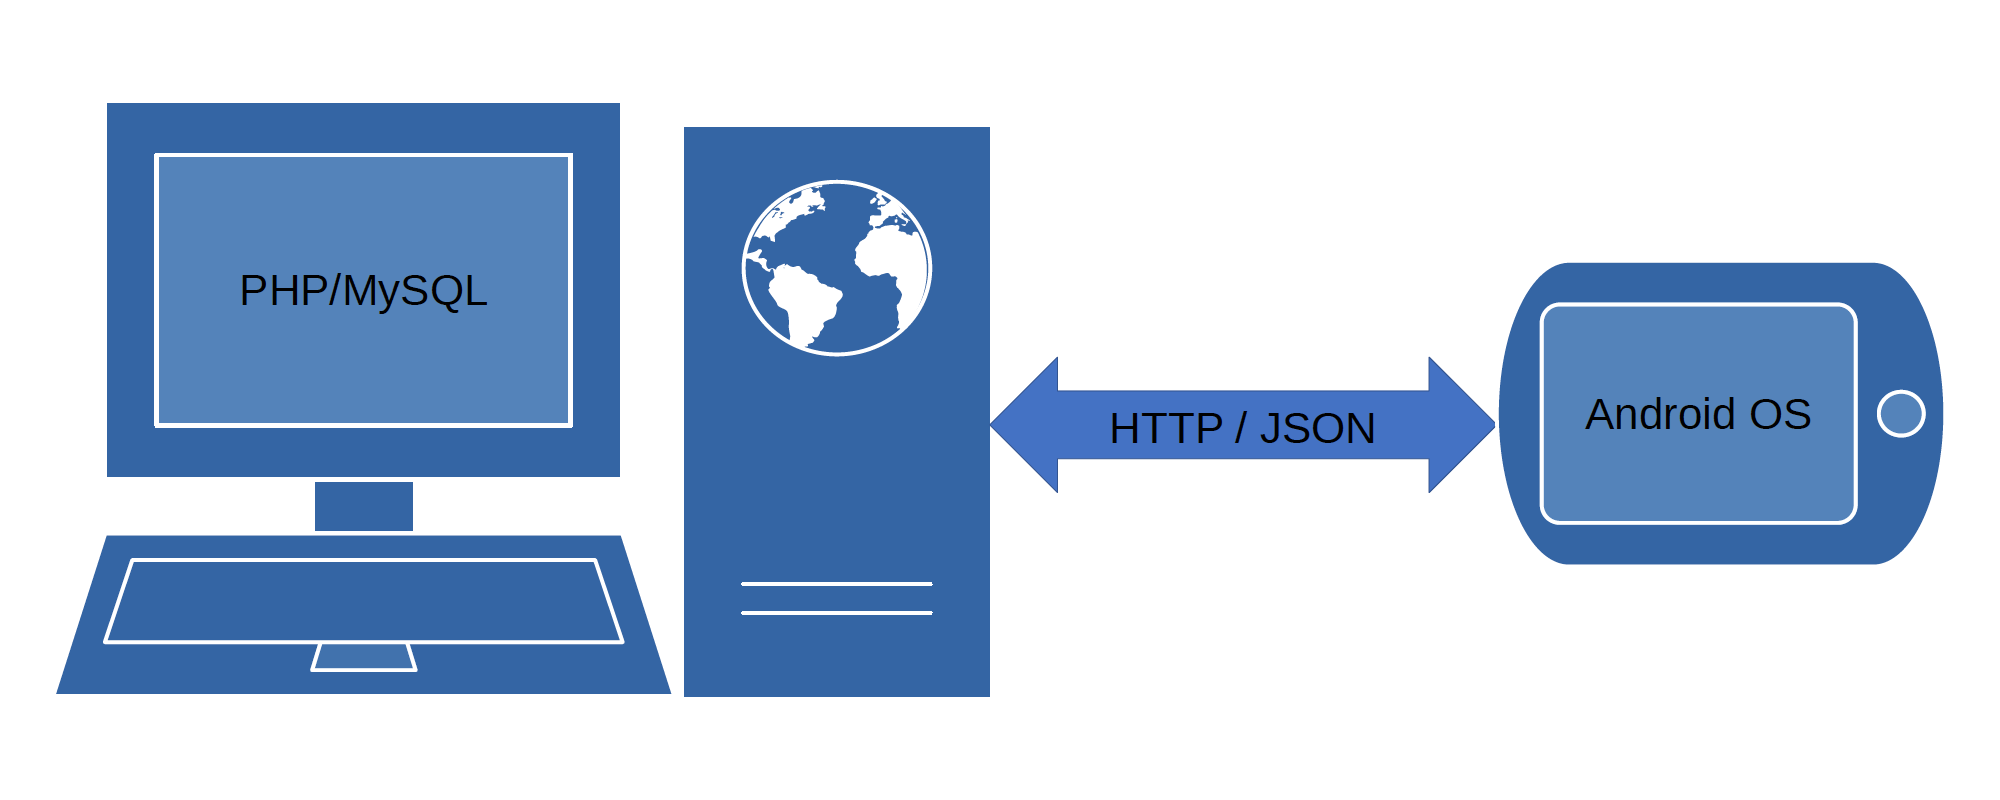
\includegraphics[width=0.8\linewidth]{fig0055.png}
  \caption{Софтуерни компоненти}
\label{fig0055}
\end{figure}

Комуникацията в системата винаги се инициира от клиентското приложение, което отправя заявки към сървъра и връща резултати. Комуникацията се извършва по протокола TCP/IP, като се използват възможностите за HTTP комуникация. По аналогия с RESTful приложенията, клиентът и сървърът обменят съобщения пакетирани с JSON. Ролята на JSON е в това информацията да бъде предавана по мрежата в структуриран вид. Възможна е реализация и с XML, но JSON е значително по-добре оптимизиран за комуникация между машини. XML намира по-широко приложение там където е нужна човешка намеса за описване на данните. JSON има и предимството, че обемът служебна информация е значително по-малък в сравнение с XML. 

От страната на клиента, стои Android OS приложение, разработено към настоящия дисертационен труд, което има основната задача да извършва разпределените изчисления и да докладва получените резултати на отдалечения сървър. Сървърното приложение не е част от настоящия дисертационен труд, а се използва на база на предходна разработка в ИИКТ-БАН \cite{Balabanov-04}. 

Изборът на мобилни устройства с операционна система Android OS е направен, тъй като тези устройства са много разпространени, със значителен пазарен дял, ядрото на операционната система е Linux базирано, а множество нейни компоненти са с отворен код. От значение е и цената на мобилните устройства, тъй като прекият конкурент iOS, на компанията Apple, поддържа значително по-високи цени. При дарените ресурси за разпределени изчисления е от съществено значение крайните потребители да могат да си позволят цената на изчислителните ресурси. Сериозно предимство на Android OS е и факта, че поддържа програмния език Java. По настояще, Java е най-широко използвания програмен език, което го прави изключително подходящ от гледна точка на човешки ресурси, при евентуално разрастване на проекта. В последните години се забелязва много силно наложена тенденция езикът Java да бъде подменен в Android OS с езика Kotlin, но този процес би отнел твърде много време. Предимство на програмния език Java е и това, че той широко се използва не само за програмиране на мобилни приложения, но и на множество други видове софтуер. За сравнение, езиците Objective-C и Swift, на компанията Apple, далеч не се използват толкова много, извън продуктите на самата компания. Това ограничение би довело до сериозни проблеми при търсенето на програмисти за мобилни устройства базирани на операционната система iOS. 

\section{Модулна организация на мобилното приложение}


